%! Author = itgramic
%! Date = 26.01.24

% Preamble
\subsubsection{Monolitische Umgebung}
\subsubsection{Kubernetes}
\begin{flushleft}
    Um ein minimales, dem Produktiven möglichst nahes Enviroment für die evaluation zu erhalten, wurde folgendes Setting ausgewählt:
    \begin{figure}[H]
        \centering
        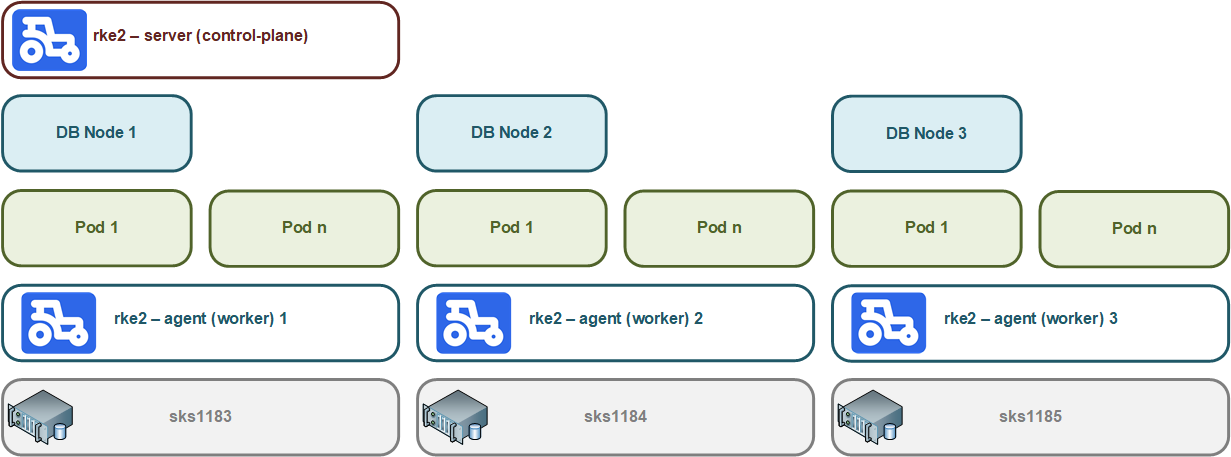
\includegraphics[width=1\linewidth]{source/implementation/evaluation/platforms/evaluation_enviroment_rke2}
        \caption{Kubernetes - Evaluations-Enviroment}
        \label{fig:k8s_evalution_enviroment}
    \end{figure}
\end{flushleft}
\begin{flushleft}
    Die genauen Spezifikationen sind wie folgt:
    \begin{table}[H]
    \begin{tabular}{ll}
    \textbf{Linux Distribution}                & Debian 11              \\
    \textbf{Kubernetes Runtime}                & rke2                   \\
    \textbf{Container-Enviroment}              & containerd             \\
    \textbf{Container Network Interface (CNI)} & cilium                 \\
    \textbf{Cloud Native Storage (CNS)}        & local-path-provisioner
    \end{tabular}
    \caption{Evaluations settings}
    \label{tab:evaluation-setting}
    \end{table}
\end{flushleft}